\section{Semi-Infinite Uniform Source}
This case is also an evaluation of an analytic function, but can't be exactly represented by a finite polynomial expansion.  The solution models the mono-energetic neutron flux at a point inside a 1D semi-infinite homogenous absorbing medium with a uniform source.  The governing PDE for this equation is
\begin{equation}
-D\ddrv{\phi}{x}+\Sigma_a\phi = S,
\end{equation}
and its solution is
\begin{equation}
\phi(S,D,x,\Sigma_a)=\frac{S}{\Sigma_a}\left(1-e^{-x/L}\right),
\end{equation}
\begin{equation}
L^2\equiv \frac{D}{\Sigma_a}.
\end{equation}
where $S$ is the uniform source, $\Sigma_a$ is the material's macroscopic absorption cross section, $D$ is the material's diffusion coefficient, $x$ is a distance into the medium from the boundary, and $\phi$ is the neutron flux.  

\subsection{Monovariate}
Restated in the form used by PCESC,
\begin{equation}
U(p;\theta) = \frac{S}{\theta}\left(1-e^{-\sqrt{\theta} x/\sqrt{D}}\right),
\end{equation}
where $p=(S,D,x)$ and $\theta=\Sigma_a$.  
We consider the cases when the absorption cross section $\theta$ has a uniform distribution as well as a normal distribution.   For both cases, parameters $p$ are as follows.
\begin{align}
S &= 1.0 \text{ n/cm}^2\text{/s},\\
D &= 0.5 \text{ /cm},\\
x &= 2.0 \text{ cm}.
\end{align}
We allow $\Sigma_a$ to vary uniformly as $\Sigma_a\in[0.5,1]$ or normally as $\Sigma_a\in\mathcal{N}(0.75,0.15)$ and quantify the uncertainty using PCESC as well as Monte Carlo sampling.
For increasing orders of expansion, the mean and variance obtained are shown along with the run time and are shown in Tables \ref{tab:source uni} and \ref{tab:source norm}.
\begin{table}
\begin{center}
\begin{tabular}{c c|l l}
type & runs/order & mean & variance \\ \hline
MC & $1\times10^6$ & 1.26069628111 & 0.0632432419713\\
SC & 2 & 1.25774207229 & 0.0495341371244 \\
SC & 4 & 1.26064320417 & 0.0604388749588 \\
SC & 8 & 1.26108375978 & 0.0637370898233\\
SC & 16 & 1.26112339681 & 0.0639754882641
\end{tabular}
\end{center}
\caption{Statistics for Source Problem with Uniform Uncertainty}
\label{tab:source uni}
\end{table}

\begin{table}[h!]
\begin{center}
\begin{tabular}{c c|l l| r}
type & runs/order & mean & variance & run time (sec) \\ \hline
MC & $1\times10^6$ & 1.24922240195 & 0.0488719424418 & 366.31\\
SC & 2 & 1.2547221522 & 0 & 2.08 \\
SC & 4 & 1.25569029702 & 0.049198975952 & 3.11 \\
SC & 8 & 1.25569096924 & 0.0492316191443 & 4.74\\
SC & 16 & 1.25569096924 & 0.0492316191611 & 6.88
\end{tabular}
\end{center}
\caption{Statistics for Source Problem with Normal Uncertainty}
\label{tab:source norm}
\end{table}

\begin{figure}[h]
\centering
  \begin{subfigure}[b]{0.45 \textwidth}
   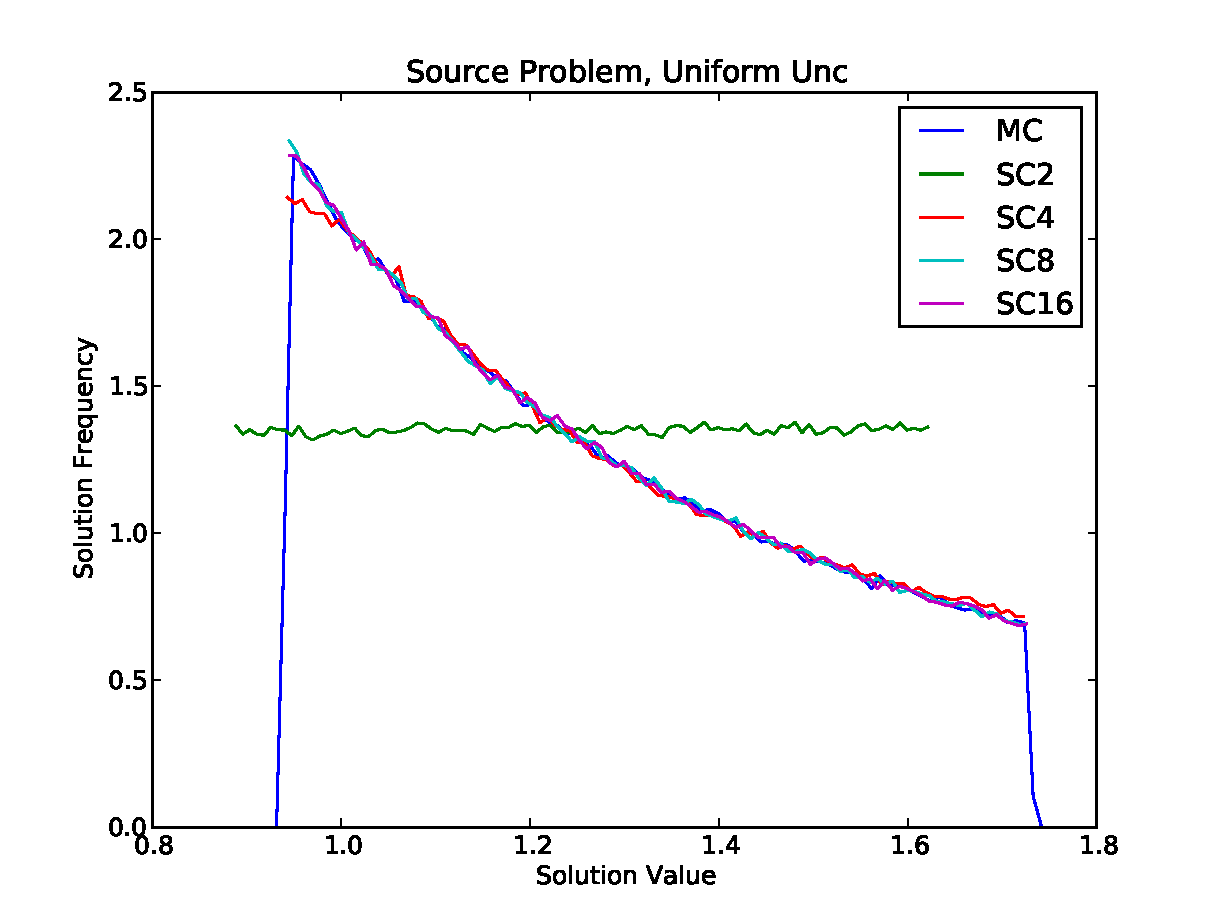
\includegraphics[width=\textwidth]{../graphics/source_uniform_pdfs}
   \caption{Uniform PDFs}
      \label{uni}
  \end{subfigure}
  \begin{subfigure}[b]{0.45\textwidth}
   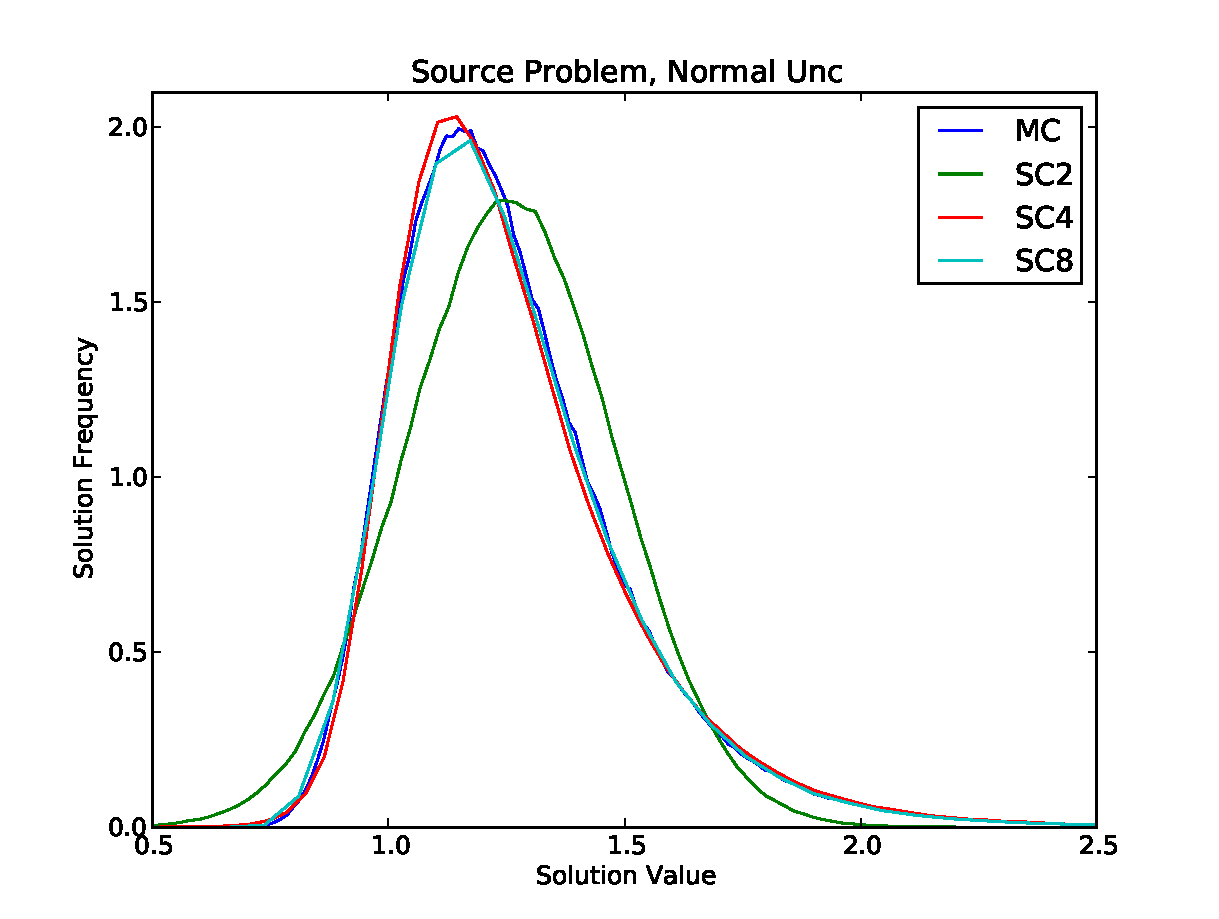
\includegraphics[width=\textwidth]{../graphics/source_normal_pdfs}
   \caption{Normal PDFs}
      \label{norm}
  \end{subfigure}
\caption{Source Problem Solution Distributions}
\label{fig:sourcepdfs}
\end{figure}

The PDFs were obtained by Monte Carlo sampling of the ROM for the PCESC cases, and obtained directly for the Monte Carlo case, shown in Fig. \ref{fig:sourcepdfs}.  The x-axis is the value of the scalar flux, and the y-axis is the probability of obtaining a particular flux.

\subsection{Bivariate}
In addition to the absorption cross section, we introduce uncertainty in the location at which the flux is measured.  For example, the exact absorption properties of a medium are unknown and a point detector is placed with some uncertainty.  Restating the problem,

\begin{equation}
U(p;\vb*{\theta}) = \frac{S}{\theta_1}\left(1-e^{-\sqrt{\theta_1} \theta_2/\sqrt{D}}\right),
\end{equation}
where $p=(S,D)$ and $\vb*{\theta}=[\theta_1,\theta_2]=[\Sigma_a,x]$.  
We consider two cases: when $\theta_1\sim\mathcal{U}(0.5,1),\theta_2\sim\mathcal{U}(1.5,2.5)$; as well when $\theta_1\sim\mathcal{N}(0.75,0.15^2),\theta_2\sim\mathcal{N}(TODO,TODO)$.   For both cases, parameters $p$ are as follows.
\begin{align}
S &= 1.0 \text{ n/cm}^2\text{/s},\\
D &= 0.5 \text{ /cm}.
\end{align}
We quantify the uncertainty using PCESC as well as Monte Carlo sampling.
For increasing orders of expansion, the mean and variance obtained are shown in Tables \ref{tab:2v source uni} and \ref{tab:2v source norm}.  The PDFs were obtained by Monte Carlo sampling of the ROM for the PCESC cases, and obtained directly for the Monte Carlo case, shown in Fig. \ref{fig:2v sourcepdfs}.  The x-axis is the value of the scalar flux, and the y-axis is the probability of obtaining a particular flux.
\begin{table}
\begin{center}
\begin{tabular}{c c|l l}
type & order($\Sigma_a,x$) & mean & variance \\ \hline
MC & $1\times10^6$ & 1.24791828682 & 0.0508287413676\\
SC & (2,2) & 1.24804231569 & 0.0506451101763 \\
SC & (2,4) & 1.24804212351 & 0.0506466208388\\
SC & (4,2) & 1.24806746049 & 0.0507934845282\\
SC & (4,4) & 1.24806726831 & 0.0507949951904 \\
\end{tabular}
\end{center}
\caption{Statistics for Source Problem with Bivariate Uniform Uncertainty}
\label{tab:2v source uni}
\end{table}

\begin{table}[h!]
\begin{center}
\begin{tabular}{c c|l l}
type & runs/order & mean & variance \\ \hline
MC & $1\times10^6$ &  & \\
SC & (2,2)     &  &  \\
SC & (4,4)     &  &  \\
SC & (8,8)     &  & \\
SC & (16,16) &  & 
\end{tabular}
\end{center}
\caption{Statistics for Source Problem with Bivariate Normal Uncertainty}
\label{tab:2v source norm}
\end{table}

\begin{figure}[h]
\centering
  \begin{subfigure}[b]{0.45 \textwidth}
   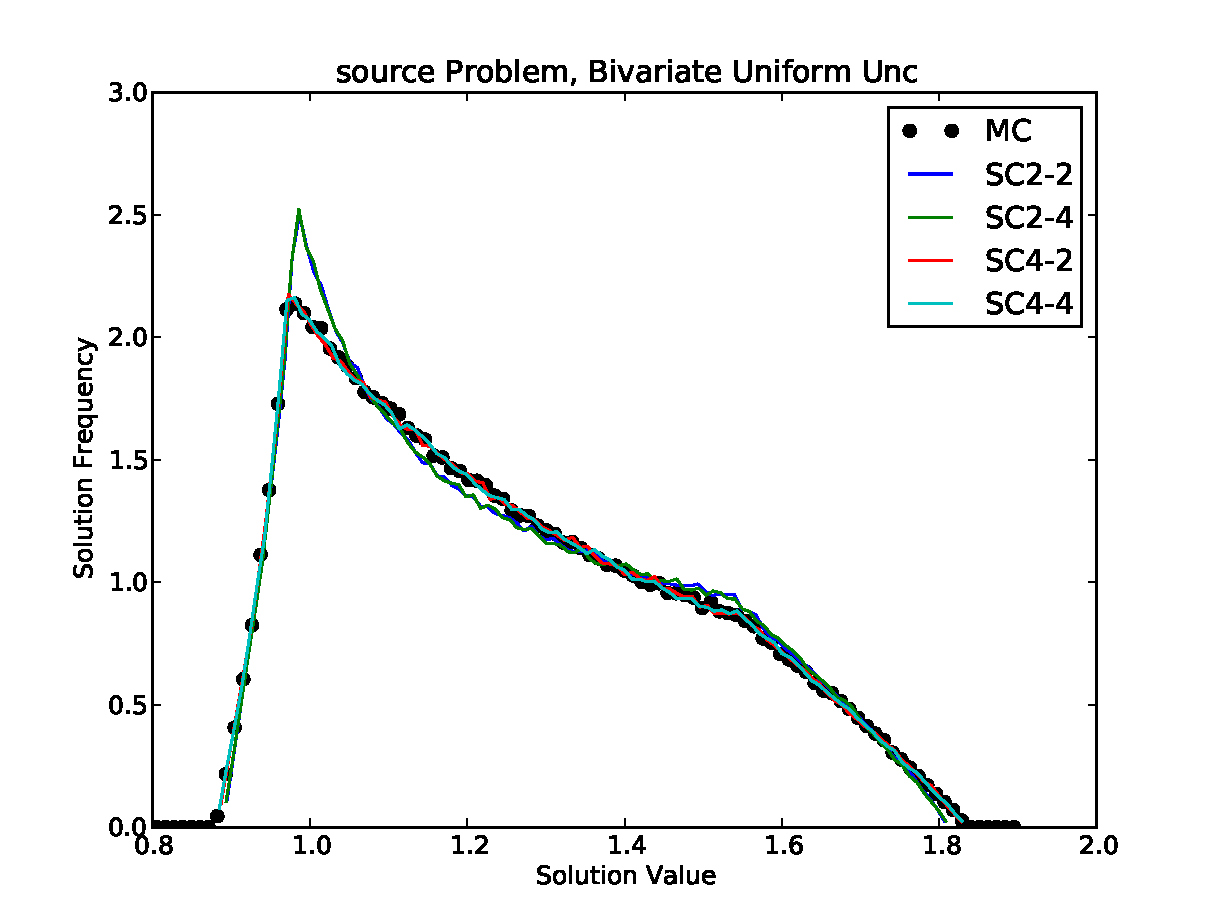
\includegraphics[width=\textwidth]{../graphics/source_2v_uniform_pdfs}
   \caption{Uniform PDFs}
      \label{uni}
  \end{subfigure}
  \begin{subfigure}[b]{0.45\textwidth}
   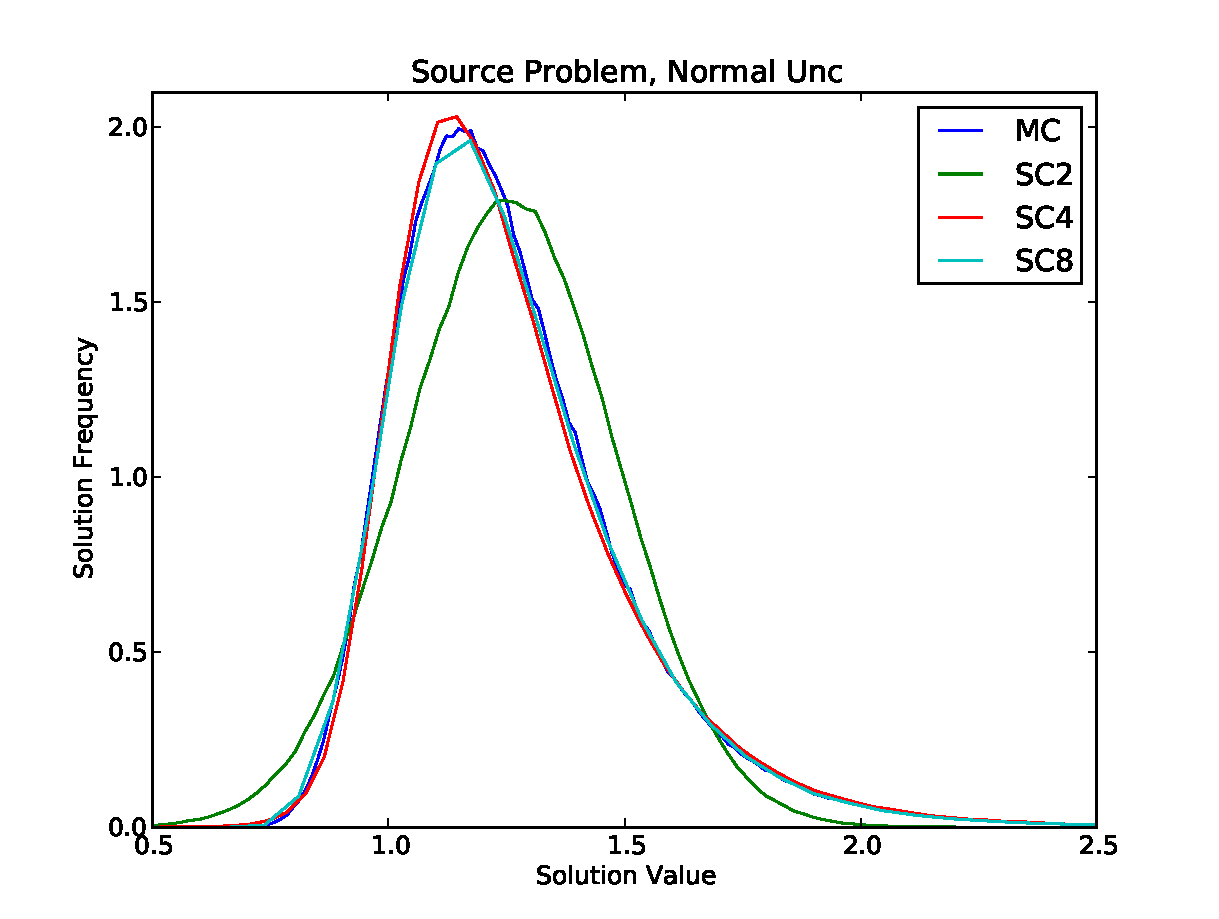
\includegraphics[width=\textwidth]{../graphics/source_normal_pdfs}
   \caption{PLACEHOLDERNormal PDFs}
      \label{norm}
  \end{subfigure}
\caption{Bivariate Source Problem Solution Distributions}
\label{fig:2v sourcepdfs}
\end{figure}


%\begin{table}
%\begin{center}
%\begin{tabular}{c c|l l| r}
%type & runs/order & mean & variance & run time (sec) \\ \hline
%MC & 1\times10^6 &  &  & \\
%SC & 2 & & & \\
%SC & 4 & & & \\
%SC & 8 & & & \\
%SC & 16 & & &
%\end{tabular}
%\end{center}
%\caption{}
%\label{}
%\end{table}
%
%\begin{figure}[h!]
%\centering
%   \includegraphics[width=\textwidth]{../graphics/}
%   \label{}
%   \caption{}
%\end{figure}
